
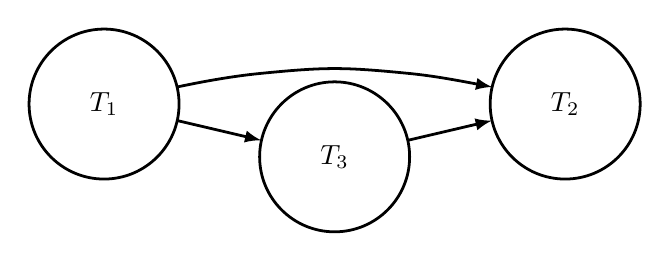
\begin{tikzpicture}[>=latex,line join=bevel,]
  \pgfsetlinewidth{1bp}
%%
\pgfsetcolor{black}
  % Edge: T_1 -> T_2
  \draw [->] (53.308bp,52.149bp) .. controls (62.587bp,54.114bp) and (73.213bp,56.031bp)  .. (83bp,57bp) .. controls (106.88bp,59.365bp) and (113.12bp,59.365bp)  .. (137bp,57bp) .. controls (143.42bp,56.364bp) and (150.21bp,55.32bp)  .. (166.69bp,52.149bp);
  % Edge: T_3 -> T_2
  \draw [->] (136.63bp,33.012bp) .. controls (142.89bp,34.481bp) and (149.71bp,36.081bp)  .. (166.54bp,40.027bp);
  % Edge: T_1 -> T_3
  \draw [->] (53.629bp,39.988bp) .. controls (59.895bp,38.519bp) and (66.712bp,36.919bp)  .. (83.538bp,32.973bp);
  % Node: T_2
\begin{scope}
  \definecolor{strokecol}{rgb}{0.0,0.0,0.0};
  \pgfsetstrokecolor{strokecol}
  \draw (193bp,46bp) ellipse (27bp and 27bp);
  \draw (193bp,46bp) node {$T_2$};
\end{scope}
  % Node: T_3
\begin{scope}
  \definecolor{strokecol}{rgb}{0.0,0.0,0.0};
  \pgfsetstrokecolor{strokecol}
  \draw (110bp,27bp) ellipse (27bp and 27bp);
  \draw (110bp,27bp) node {$T_3$};
\end{scope}
  % Node: T_1
\begin{scope}
  \definecolor{strokecol}{rgb}{0.0,0.0,0.0};
  \pgfsetstrokecolor{strokecol}
  \draw (27bp,46bp) ellipse (27bp and 27bp);
  \draw (27bp,46bp) node {$T_1$};
\end{scope}
%
\end{tikzpicture}

